\documentclass[tikz]{standalone}
\usetikzlibrary{arrows, positioning}
\tikzset{
  treenode/.style = {align=center, inner sep=1pt, text centered,
    font=\sffamily},
  bst/.style = {treenode, circle, black, font=\sffamily\bfseries, draw=black, text width=2em}, 
  sst/.style = {treenode, circle, black, font=\sffamily\bfseries, draw=red, text width=2em}, 
  txt/.style = {text width=1.5em, red},
  redline/.style={edge from parent/.style={red,very thick,-latex, draw}},
  rugularline/.style={edge from parent/.style={black, line width=0.2mm, draw}},
  noline/.style={edge from parent/.style={black, line width=0.2mm}},
}
\begin{document}
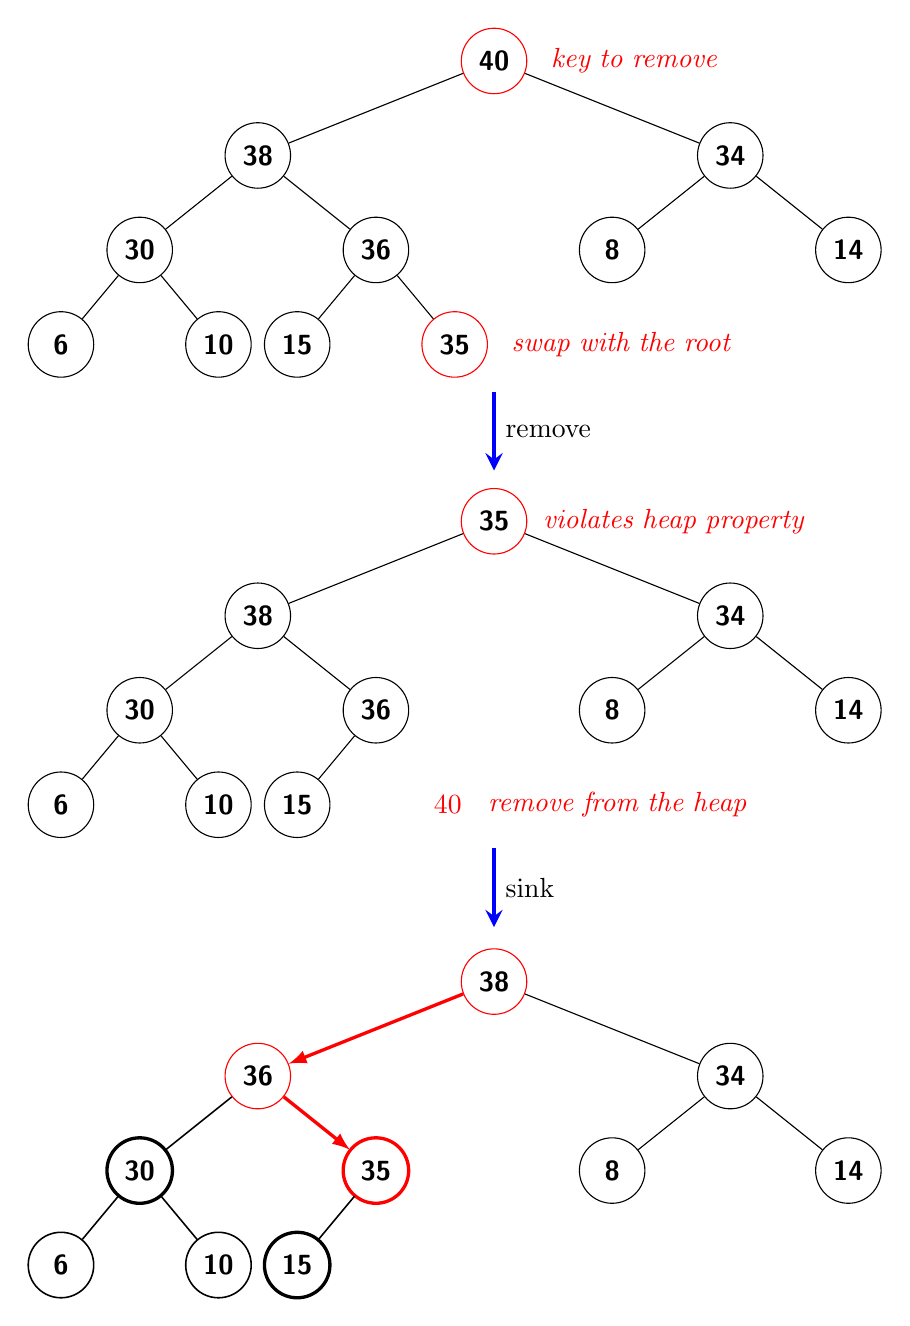
\begin{tikzpicture}[level/.style={sibling distance = 6cm/#1,
  level distance = 1.2cm}] 

\node [sst] (n1) {40}
    child {node [bst] {38}
        child {node [bst] {30}
            child {node [bst] {6}}
            child {node [bst] {10}}
        }
        child  {node [bst] {36}
            child {node [bst] {15}}
            child {node (key35) [sst] {35}}
        }
    }
    child { node [bst] {34}
        child{node [bst] {8}}
        child{node [bst] {14}}
    }
;
\node [right, txt, text width=4cm, xshift=6mm] at (n1) {\textit{key to remove}};
\node [right, txt, text width=4cm, xshift=6mm] at (key35) {\textit{swap with the root}};

\draw [stealth-, line width=0.6mm, draw=blue](0,-5.2) -- (0,-4.2)node[midway,right,shape=rectangle,draw=none]{remove};

\node [sst, below=of n1, yshift=-4cm] (2n1) {35}
    child {node [bst] {38}
        child {node [bst] {30}
            child {node [bst] {6}}
            child {node [bst] {10}}
        }
        child  {node [bst] {36}
            child {node [bst] {15}}
            child [noline] {node (2key40) [txt] {40}}
        }
    }
    child { node [bst] {34}
        child{node [bst] {8}}
        child{node [bst] {14}}
    }
;
\node [right, txt, text width=4cm, xshift=3mm] at (2key40) {\textit{remove from the heap}};
\node [right, txt, text width=4cm, xshift=5mm] at (2n1) {\textit{violates heap property}};

\draw [stealth-, line width=0.6mm, draw=blue](0,-11) -- (0,-10)node[midway,right,shape=rectangle,draw=none]{sink};

\node [sst, below=of 2n1, yshift=-4cm] (3n1) {38}
    child [redline] {node [sst] {36}
        child [rugularline] {node [bst] {30}
            child {node [bst] {6}}
            child {node [bst] {10}}
        }
        child  {node [sst] {35}
            child [rugularline] {node [bst] {15}}
            child [noline] {node {}}
        }
    }
    child { node [bst] {34}
        child{node [bst] {8}}
        child{node [bst] {14}}
    }
;

\end{tikzpicture}
\end{document}